\documentclass[1p]{elsarticle_modified}
%\bibliographystyle{elsarticle-num}

%\usepackage[colorlinks]{hyperref}
%\usepackage{abbrmath_seonhwa} %\Abb, \Ascr, \Acal ,\Abf, \Afrak
\usepackage{amsfonts}
\usepackage{amssymb}
\usepackage{amsmath}
\usepackage{amsthm}
\usepackage{scalefnt}
\usepackage{amsbsy}
\usepackage{kotex}
\usepackage{caption}
\usepackage{subfig}
\usepackage{color}
\usepackage{graphicx}
\usepackage{xcolor} %% white, black, red, green, blue, cyan, magenta, yellow
\usepackage{float}
\usepackage{setspace}
\usepackage{hyperref}

\usepackage{tikz}
\usetikzlibrary{arrows}

\usepackage{multirow}
\usepackage{array} % fixed length table
\usepackage{hhline}

%%%%%%%%%%%%%%%%%%%%%
\makeatletter
\renewcommand*\env@matrix[1][\arraystretch]{%
	\edef\arraystretch{#1}%
	\hskip -\arraycolsep
	\let\@ifnextchar\new@ifnextchar
	\array{*\c@MaxMatrixCols c}}
\makeatother %https://tex.stackexchange.com/questions/14071/how-can-i-increase-the-line-spacing-in-a-matrix
%%%%%%%%%%%%%%%

\usepackage[normalem]{ulem}

\newcommand{\msout}[1]{\ifmmode\text{\sout{\ensuremath{#1}}}\else\sout{#1}\fi}
%SOURCE: \msout is \stkout macro in https://tex.stackexchange.com/questions/20609/strikeout-in-math-mode

\newcommand{\cancel}[1]{
	\ifmmode
	{\color{red}\msout{#1}}
	\else
	{\color{red}\sout{#1}}
	\fi
}

\newcommand{\add}[1]{
	{\color{blue}\uwave{#1}}
}

\newcommand{\replace}[2]{
	\ifmmode
	{\color{red}\msout{#1}}{\color{blue}\uwave{#2}}
	\else
	{\color{red}\sout{#1}}{\color{blue}\uwave{#2}}
	\fi
}

\newcommand{\Sol}{\mathcal{S}} %segment
\newcommand{\D}{D} %diagram
\newcommand{\A}{\mathcal{A}} %arc


%%%%%%%%%%%%%%%%%%%%%%%%%%%%%5 test

\def\sl{\operatorname{\textup{SL}}(2,\Cbb)}
\def\psl{\operatorname{\textup{PSL}}(2,\Cbb)}
\def\quan{\mkern 1mu \triangleright \mkern 1mu}

\theoremstyle{definition}
\newtheorem{thm}{Theorem}[section]
\newtheorem{prop}[thm]{Proposition}
\newtheorem{lem}[thm]{Lemma}
\newtheorem{ques}[thm]{Question}
\newtheorem{cor}[thm]{Corollary}
\newtheorem{defn}[thm]{Definition}
\newtheorem{exam}[thm]{Example}
\newtheorem{rmk}[thm]{Remark}
\newtheorem{alg}[thm]{Algorithm}

\newcommand{\I}{\sqrt{-1}}
\begin{document}

%\begin{frontmatter}
%
%\title{Boundary parabolic representations of knots up to 8 crossings}
%
%%% Group authors per affiliation:
%\author{Yunhi Cho} 
%\address{Department of Mathematics, University of Seoul, Seoul, Korea}
%\ead{yhcho@uos.ac.kr}
%
%
%\author{Seonhwa Kim} %\fnref{s_kim}}
%\address{Center for Geometry and Physics, Institute for Basic Science, Pohang, 37673, Korea}
%\ead{ryeona17@ibs.re.kr}
%
%\author{Hyuk Kim}
%\address{Department of Mathematical Sciences, Seoul National University, Seoul 08826, Korea}
%\ead{hyukkim@snu.ac.kr}
%
%\author{Seokbeom Yoon}
%\address{Department of Mathematical Sciences, Seoul National University, Seoul, 08826,  Korea}
%\ead{sbyoon15@snu.ac.kr}
%
%\begin{abstract}
%We find all boundary parabolic representation of knots up to 8 crossings.
%
%\end{abstract}
%\begin{keyword}
%    \MSC[2010] 57M25 
%\end{keyword}
%
%\end{frontmatter}

%\linenumbers
%\tableofcontents
%
\newcommand\colored[1]{\textcolor{white}{\rule[-0.35ex]{0.8em}{1.4ex}}\kern-0.8em\color{red} #1}%
%\newcommand\colored[1]{\textcolor{white}{ #1}\kern-2.17ex	\textcolor{white}{ #1}\kern-1.81ex	\textcolor{white}{ #1}\kern-2.15ex\color{red}#1	}

{\Large $\underline{12a_{1204}~(K12a_{1204})}$}

\setlength{\tabcolsep}{10pt}
\renewcommand{\arraystretch}{1.6}
\vspace{1cm}\begin{tabular}{m{100pt}>{\centering\arraybackslash}m{274pt}}
\multirow{5}{120pt}{
	\centering
	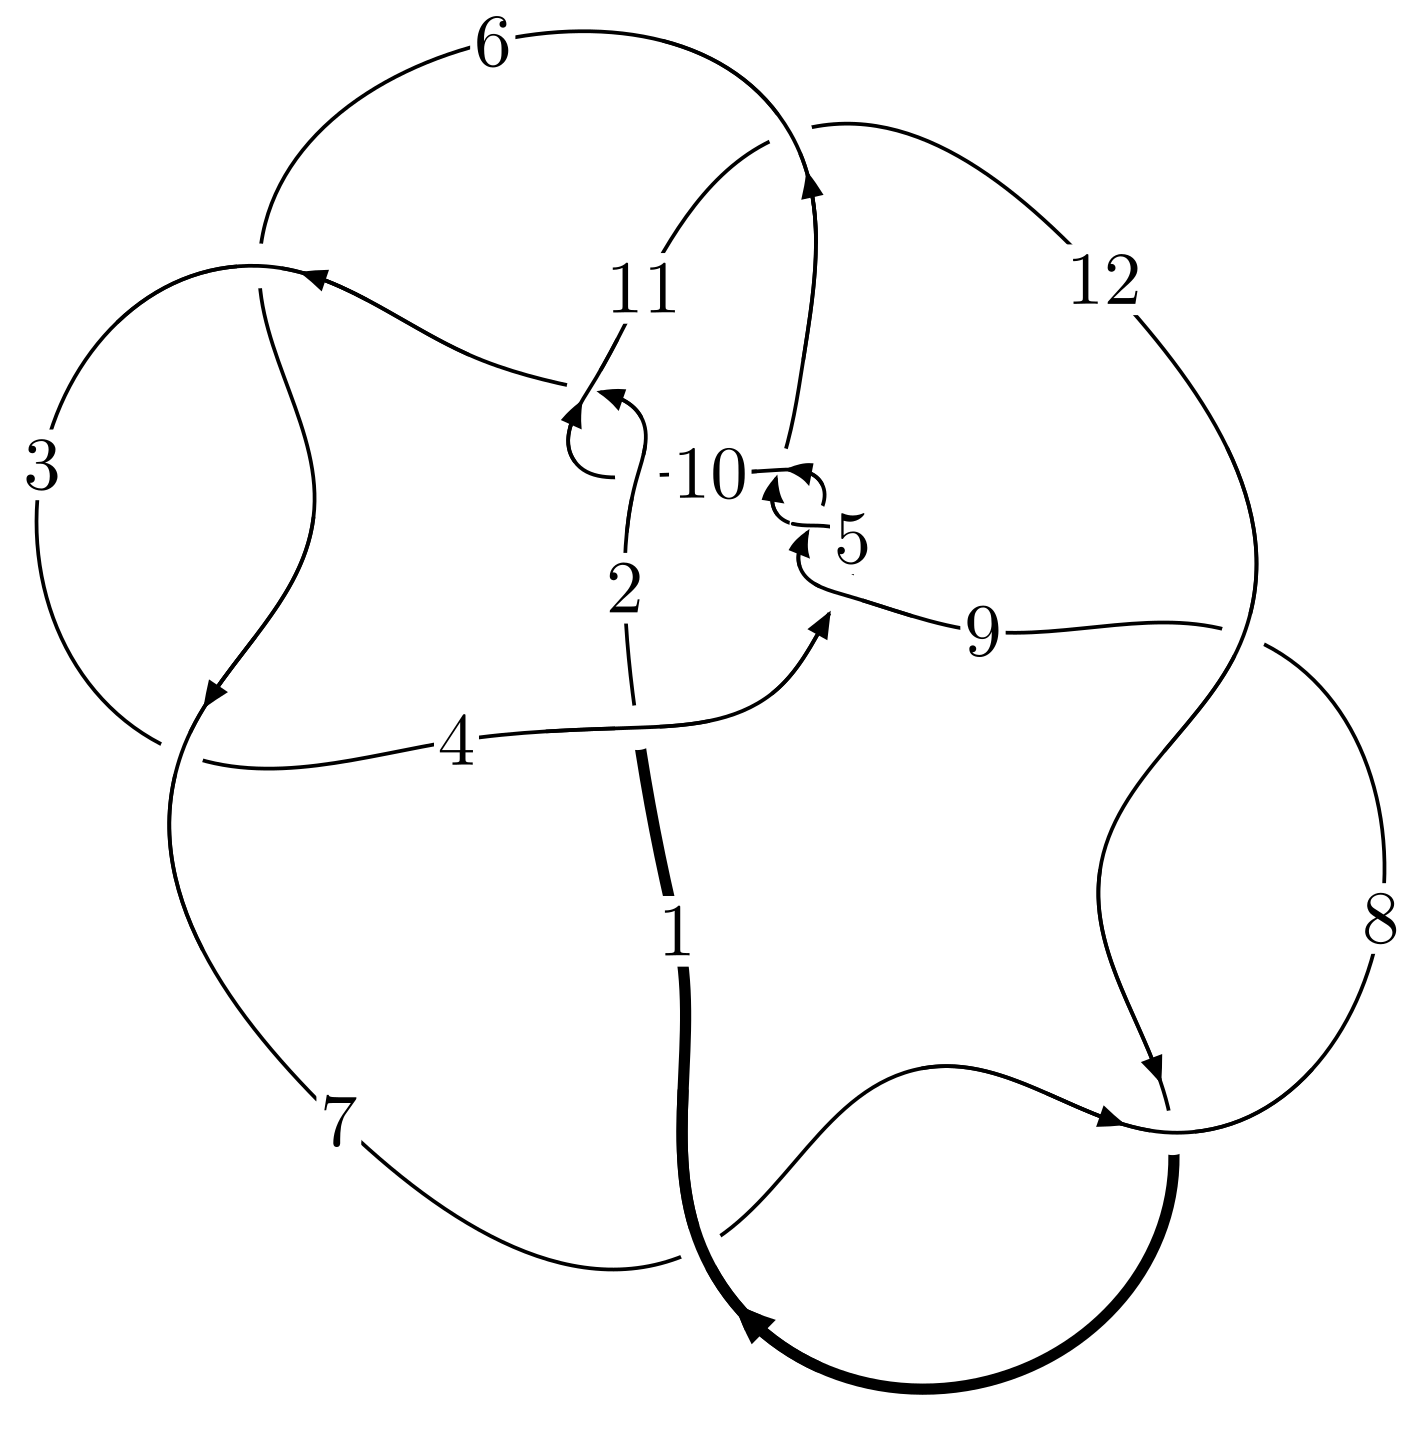
\includegraphics[width=112pt]{../../../GIT/diagram.site/Diagrams/png/2005_12a_1204.png}\\
\ \ \ A knot diagram\footnotemark}&
\allowdisplaybreaks
\textbf{Linearized knot diagam} \\
\cline{2-2}
 &
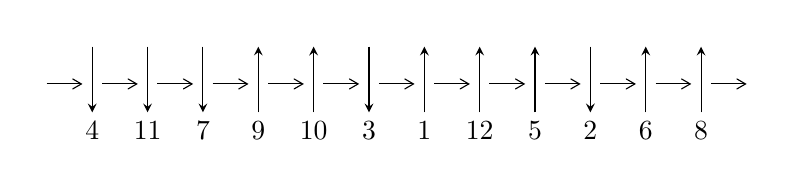
\begin{tikzpicture}[x=20pt, y=17pt]
	% nodes
	\node (C0) at (0, 0) {};
	\node (C1) at (1, 0) {};
	\node (C1U) at (1, +1) {};
	\node (C1D) at (1, -1) {4};

	\node (C2) at (2, 0) {};
	\node (C2U) at (2, +1) {};
	\node (C2D) at (2, -1) {11};

	\node (C3) at (3, 0) {};
	\node (C3U) at (3, +1) {};
	\node (C3D) at (3, -1) {7};

	\node (C4) at (4, 0) {};
	\node (C4U) at (4, +1) {};
	\node (C4D) at (4, -1) {9};

	\node (C5) at (5, 0) {};
	\node (C5U) at (5, +1) {};
	\node (C5D) at (5, -1) {10};

	\node (C6) at (6, 0) {};
	\node (C6U) at (6, +1) {};
	\node (C6D) at (6, -1) {3};

	\node (C7) at (7, 0) {};
	\node (C7U) at (7, +1) {};
	\node (C7D) at (7, -1) {1};

	\node (C8) at (8, 0) {};
	\node (C8U) at (8, +1) {};
	\node (C8D) at (8, -1) {12};

	\node (C9) at (9, 0) {};
	\node (C9U) at (9, +1) {};
	\node (C9D) at (9, -1) {5};

	\node (C10) at (10, 0) {};
	\node (C10U) at (10, +1) {};
	\node (C10D) at (10, -1) {2};

	\node (C11) at (11, 0) {};
	\node (C11U) at (11, +1) {};
	\node (C11D) at (11, -1) {6};

	\node (C12) at (12, 0) {};
	\node (C12U) at (12, +1) {};
	\node (C12D) at (12, -1) {8};
	\node (C13) at (13, 0) {};

	% arrows
	\draw[->,>={angle 60}]
	(C0) edge (C1) (C1) edge (C2) (C2) edge (C3) (C3) edge (C4) (C4) edge (C5) (C5) edge (C6) (C6) edge (C7) (C7) edge (C8) (C8) edge (C9) (C9) edge (C10) (C10) edge (C11) (C11) edge (C12) (C12) edge (C13) ;	\draw[->,>=stealth]
	(C1U) edge (C1D) (C2U) edge (C2D) (C3U) edge (C3D) (C4D) edge (C4U) (C5D) edge (C5U) (C6U) edge (C6D) (C7D) edge (C7U) (C8D) edge (C8U) (C9D) edge (C9U) (C10U) edge (C10D) (C11D) edge (C11U) (C12D) edge (C12U) ;
	\end{tikzpicture} \\
\hhline{~~} \\& 
\textbf{Solving Sequence} \\ \cline{2-2} 
 &
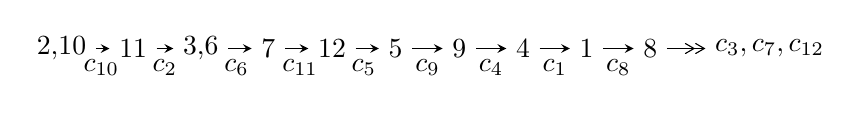
\begin{tikzpicture}[x=23pt, y=7pt]
	% node
	\node (A0) at (-1/8, 0) {2,10};
	\node (A1) at (1, 0) {11};
	\node (A2) at (33/16, 0) {3,6};
	\node (A3) at (25/8, 0) {7};
	\node (A4) at (33/8, 0) {12};
	\node (A5) at (41/8, 0) {5};
	\node (A6) at (49/8, 0) {9};
	\node (A7) at (57/8, 0) {4};
	\node (A8) at (65/8, 0) {1};
	\node (A9) at (73/8, 0) {8};
	\node (C1) at (1/2, -1) {$c_{10}$};
	\node (C2) at (3/2, -1) {$c_{2}$};
	\node (C3) at (21/8, -1) {$c_{6}$};
	\node (C4) at (29/8, -1) {$c_{11}$};
	\node (C5) at (37/8, -1) {$c_{5}$};
	\node (C6) at (45/8, -1) {$c_{9}$};
	\node (C7) at (53/8, -1) {$c_{4}$};
	\node (C8) at (61/8, -1) {$c_{1}$};
	\node (C9) at (69/8, -1) {$c_{8}$};
	\node (A10) at (11, 0) {$c_{3},c_{7},c_{12}$};

	% edge
	\draw[->,>=stealth]	
	(A0) edge (A1) (A1) edge (A2) (A2) edge (A3) (A3) edge (A4) (A4) edge (A5) (A5) edge (A6) (A6) edge (A7) (A7) edge (A8) (A8) edge (A9) ;
	\draw[->>,>={angle 60}]	
	(A9) edge (A10);
\end{tikzpicture} \\ 

\end{tabular} \\

\footnotetext{
The image of knot diagram is generated by the software ``\textbf{Draw programme}" developed by Andrew Bartholomew(\url{http://www.layer8.co.uk/maths/draw/index.htm\#Running-draw}), where we modified some parts for our purpose(\url{https://github.com/CATsTAILs/LinksPainter}).
}\phantom \\ \newline 
\centering \textbf{Ideals for irreducible components\footnotemark of $X_{\text{par}}$} 
 
\begin{align*}
I^u_{1}&=\langle 
4.67618\times10^{190} u^{79}+2.29826\times10^{191} u^{78}+\cdots+5.15330\times10^{191} b-1.47967\times10^{191},\\
\phantom{I^u_{1}}&\phantom{= \langle  }5.17863\times10^{194} u^{79}+2.01367\times10^{195} u^{78}+\cdots+3.38572\times10^{194} a-3.88078\times10^{195},\;u^{80}+4 u^{79}+\cdots-12 u+1\rangle \\
I^u_{2}&=\langle 
- a u+b+2 a+u-1,\;3 a^2+2 a u-4 a-3 u+1,\;u^2- u+1\rangle \\
I^u_{3}&=\langle 
b,\;3 a- u+2,\;u^2- u+1\rangle \\
\\
\end{align*}
\raggedright * 3 irreducible components of $\dim_{\mathbb{C}}=0$, with total 86 representations.\\
\footnotetext{All coefficients of polynomials are rational numbers. But the coefficients are sometimes approximated in decimal forms when there is not enough margin.}
\newpage
\renewcommand{\arraystretch}{1}
\centering \section*{I. $I^u_{1}= \langle 4.68\times10^{190} u^{79}+2.30\times10^{191} u^{78}+\cdots+5.15\times10^{191} b-1.48\times10^{191},\;5.18\times10^{194} u^{79}+2.01\times10^{195} u^{78}+\cdots+3.39\times10^{194} a-3.88\times10^{195},\;u^{80}+4 u^{79}+\cdots-12 u+1 \rangle$}
\flushleft \textbf{(i) Arc colorings}\\
\begin{tabular}{m{7pt} m{180pt} m{7pt} m{180pt} }
\flushright $a_{2}=$&$\begin{pmatrix}0\\u\end{pmatrix}$ \\
\flushright $a_{10}=$&$\begin{pmatrix}1\\0\end{pmatrix}$ \\
\flushright $a_{11}=$&$\begin{pmatrix}1\\u^2\end{pmatrix}$ \\
\flushright $a_{3}=$&$\begin{pmatrix}- u\\- u^3+u\end{pmatrix}$ \\
\flushright $a_{6}=$&$\begin{pmatrix}-1.52955 u^{79}-5.94754 u^{78}+\cdots+130.269 u+11.4622\\-0.0907415 u^{79}-0.445978 u^{78}+\cdots+17.6286 u+0.287130\end{pmatrix}$ \\
\flushright $a_{7}=$&$\begin{pmatrix}-1.65356 u^{79}-6.34789 u^{78}+\cdots+128.810 u+11.4548\\-0.0338236 u^{79}-0.258688 u^{78}+\cdots+20.3603 u+0.198906\end{pmatrix}$ \\
\flushright $a_{12}=$&$\begin{pmatrix}0.665941 u^{79}+2.23325 u^{78}+\cdots-127.524 u-19.4828\\0.155254 u^{79}+0.344909 u^{78}+\cdots+1.73662 u-2.15467\end{pmatrix}$ \\
\flushright $a_{5}=$&$\begin{pmatrix}-1.43881 u^{79}-5.50156 u^{78}+\cdots+112.640 u+11.1751\\-0.0907415 u^{79}-0.445978 u^{78}+\cdots+17.6286 u+0.287130\end{pmatrix}$ \\
\flushright $a_{9}=$&$\begin{pmatrix}0.0923606 u^{79}-0.0500166 u^{78}+\cdots+123.650 u+20.7512\\-0.0594848 u^{79}-0.0792420 u^{78}+\cdots-4.89863 u+2.41543\end{pmatrix}$ \\
\flushright $a_{4}=$&$\begin{pmatrix}1.34210 u^{79}+5.18617 u^{78}+\cdots-149.249 u-11.9533\\-0.0202947 u^{79}+0.0673583 u^{78}+\cdots-22.2316 u-0.192689\end{pmatrix}$ \\
\flushright $a_{1}=$&$\begin{pmatrix}-1.65777 u^{79}-6.13193 u^{78}+\cdots+175.851 u+12.0583\\-0.266688 u^{79}-0.803074 u^{78}+\cdots+26.9199 u+0.143262\end{pmatrix}$ \\
\flushright $a_{8}=$&$\begin{pmatrix}-0.0702822 u^{79}-0.631763 u^{78}+\cdots+138.701 u+15.5114\\0.144757 u^{79}+0.784009 u^{78}+\cdots-4.02021 u+2.28039\end{pmatrix}$\\&\end{tabular}
\flushleft \textbf{(ii) Obstruction class $= -1$}\\~\\
\flushleft \textbf{(iii) Cusp Shapes $= -0.129037 u^{79}-0.380541 u^{78}+\cdots-11.6124 u+3.37199$}\\~\\
\newpage\renewcommand{\arraystretch}{1}
\flushleft \textbf{(iv) u-Polynomials at the component}\newline \\
\begin{tabular}{m{50pt}|m{274pt}}
Crossings & \hspace{64pt}u-Polynomials at each crossing \\
\hline $$\begin{aligned}c_{1}\end{aligned}$$&$\begin{aligned}
&219(219 u^{80}+1298 u^{79}+\cdots+2.36254\times10^{7} u-1524503)
\end{aligned}$\\
\hline $$\begin{aligned}c_{2},c_{10}\end{aligned}$$&$\begin{aligned}
&u^{80}+4 u^{79}+\cdots-12 u+1
\end{aligned}$\\
\hline $$\begin{aligned}c_{3},c_{6}\end{aligned}$$&$\begin{aligned}
&u^{80}+3 u^{79}+\cdots+313 u+63
\end{aligned}$\\
\hline $$\begin{aligned}c_{4},c_{5},c_{9}\end{aligned}$$&$\begin{aligned}
&u^{80}+3 u^{79}+\cdots+180 u+36
\end{aligned}$\\
\hline $$\begin{aligned}c_{7},c_{8},c_{12}\end{aligned}$$&$\begin{aligned}
&u^{80}-2 u^{79}+\cdots-2 u+1
\end{aligned}$\\
\hline $$\begin{aligned}c_{11}\end{aligned}$$&$\begin{aligned}
&219(219 u^{80}-1403 u^{79}+\cdots-226003 u+252193)
\end{aligned}$\\
\hline
\end{tabular}\\~\\
\newpage\renewcommand{\arraystretch}{1}
\flushleft \textbf{(v) Riley Polynomials at the component}\newline \\
\begin{tabular}{m{50pt}|m{274pt}}
Crossings & \hspace{64pt}Riley Polynomials at each crossing \\
\hline $$\begin{aligned}c_{1}\end{aligned}$$&$\begin{aligned}
&47961(47961 y^{80}-3172252 y^{79}+\cdots-2.97153\times10^{14} y+2.32411\times10^{12})
\end{aligned}$\\
\hline $$\begin{aligned}c_{2},c_{10}\end{aligned}$$&$\begin{aligned}
&y^{80}-44 y^{79}+\cdots-392 y+1
\end{aligned}$\\
\hline $$\begin{aligned}c_{3},c_{6}\end{aligned}$$&$\begin{aligned}
&y^{80}-69 y^{79}+\cdots+7367 y+3969
\end{aligned}$\\
\hline $$\begin{aligned}c_{4},c_{5},c_{9}\end{aligned}$$&$\begin{aligned}
&y^{80}-75 y^{79}+\cdots+9648 y+1296
\end{aligned}$\\
\hline $$\begin{aligned}c_{7},c_{8},c_{12}\end{aligned}$$&$\begin{aligned}
&y^{80}+76 y^{79}+\cdots-72 y+1
\end{aligned}$\\
\hline $$\begin{aligned}c_{11}\end{aligned}$$&$\begin{aligned}
&47961\\
&\cdot(47961 y^{80}+610535 y^{79}+\cdots+286076439375 y+63601309249)
\end{aligned}$\\
\hline
\end{tabular}\\~\\
\newpage\flushleft \textbf{(vi) Complex Volumes and Cusp Shapes}
$$\begin{array}{c|c|c}  
\text{Solutions to }I^u_{1}& \I (\text{vol} + \sqrt{-1}CS) & \text{Cusp shape}\\
 \hline 
\begin{aligned}
u &= -0.983733 + 0.200765 I \\
a &= \phantom{-}0.406326 - 1.062540 I \\
b &= -0.210455 - 0.410314 I\end{aligned}
 & -1.68334 + 0.90111 I & \phantom{-0.000000 } 0 \\ \hline\begin{aligned}
u &= -0.983733 - 0.200765 I \\
a &= \phantom{-}0.406326 + 1.062540 I \\
b &= -0.210455 + 0.410314 I\end{aligned}
 & -1.68334 - 0.90111 I & \phantom{-0.000000 } 0 \\ \hline\begin{aligned}
u &= \phantom{-}0.061105 + 1.004630 I \\
a &= \phantom{-}0.047178 - 0.295322 I \\
b &= \phantom{-}0.350818 - 0.747248 I\end{aligned}
 & -9.01085 - 6.45760 I & \phantom{-0.000000 -}0. + 5.37585 I \\ \hline\begin{aligned}
u &= \phantom{-}0.061105 - 1.004630 I \\
a &= \phantom{-}0.047178 + 0.295322 I \\
b &= \phantom{-}0.350818 + 0.747248 I\end{aligned}
 & -9.01085 + 6.45760 I & \phantom{-0.000000 } 0. - 5.37585 I \\ \hline\begin{aligned}
u &= -0.933989 + 0.285753 I \\
a &= -0.74243 - 1.63544 I \\
b &= -1.22686 - 0.73490 I\end{aligned}
 & -2.96990 + 3.39349 I & \phantom{-0.000000 } 0. - 7.61793 I \\ \hline\begin{aligned}
u &= -0.933989 - 0.285753 I \\
a &= -0.74243 + 1.63544 I \\
b &= -1.22686 + 0.73490 I\end{aligned}
 & -2.96990 - 3.39349 I & \phantom{-0.000000 -}0. + 7.61793 I \\ \hline\begin{aligned}
u &= \phantom{-}0.935699 + 0.210723 I \\
a &= \phantom{-}0.93109 - 1.46911 I \\
b &= \phantom{-}1.36724 - 0.37575 I\end{aligned}
 & \phantom{-}1.85985 - 1.63062 I & \phantom{-}6.44657 + 8.90264 I \\ \hline\begin{aligned}
u &= \phantom{-}0.935699 - 0.210723 I \\
a &= \phantom{-}0.93109 + 1.46911 I \\
b &= \phantom{-}1.36724 + 0.37575 I\end{aligned}
 & \phantom{-}1.85985 + 1.63062 I & \phantom{-}6.44657 - 8.90264 I \\ \hline\begin{aligned}
u &= \phantom{-}0.982994 + 0.345718 I \\
a &= \phantom{-}0.35044 + 2.66174 I \\
b &= -1.267870 + 0.058555 I\end{aligned}
 & -3.53605 - 1.28537 I & \phantom{-0.000000 } 0 \\ \hline\begin{aligned}
u &= \phantom{-}0.982994 - 0.345718 I \\
a &= \phantom{-}0.35044 - 2.66174 I \\
b &= -1.267870 - 0.058555 I\end{aligned}
 & -3.53605 + 1.28537 I & \phantom{-0.000000 } 0\\
 \hline 
 \end{array}$$\newpage$$\begin{array}{c|c|c}  
\text{Solutions to }I^u_{1}& \I (\text{vol} + \sqrt{-1}CS) & \text{Cusp shape}\\
 \hline 
\begin{aligned}
u &= -0.623999 + 0.842208 I \\
a &= -0.557374 + 0.473399 I \\
b &= \phantom{-}1.44059 - 0.02605 I\end{aligned}
 & \phantom{-}4.98872 + 2.13695 I & \phantom{-0.000000 } 0 \\ \hline\begin{aligned}
u &= -0.623999 - 0.842208 I \\
a &= -0.557374 - 0.473399 I \\
b &= \phantom{-}1.44059 + 0.02605 I\end{aligned}
 & \phantom{-}4.98872 - 2.13695 I & \phantom{-0.000000 } 0 \\ \hline\begin{aligned}
u &= -0.625616 + 0.709759 I \\
a &= -0.274228 - 0.231688 I \\
b &= -0.446384 - 0.021824 I\end{aligned}
 & -1.13446 + 2.26935 I & \phantom{-}7.02637 - 5.16830 I \\ \hline\begin{aligned}
u &= -0.625616 - 0.709759 I \\
a &= -0.274228 + 0.231688 I \\
b &= -0.446384 + 0.021824 I\end{aligned}
 & -1.13446 - 2.26935 I & \phantom{-}7.02637 + 5.16830 I \\ \hline\begin{aligned}
u &= \phantom{-}1.016920 + 0.278841 I \\
a &= -0.10025 - 1.49918 I \\
b &= \phantom{-}0.328162 - 0.823029 I\end{aligned}
 & -1.15386 - 3.31282 I & \phantom{-0.000000 } 0 \\ \hline\begin{aligned}
u &= \phantom{-}1.016920 - 0.278841 I \\
a &= -0.10025 + 1.49918 I \\
b &= \phantom{-}0.328162 + 0.823029 I\end{aligned}
 & -1.15386 + 3.31282 I & \phantom{-0.000000 } 0 \\ \hline\begin{aligned}
u &= \phantom{-}1.049730 + 0.159659 I \\
a &= -1.42081 - 1.29437 I \\
b &= -0.033240 - 0.406752 I\end{aligned}
 & -7.23462 + 0.23504 I & \phantom{-0.000000 } 0 \\ \hline\begin{aligned}
u &= \phantom{-}1.049730 - 0.159659 I \\
a &= -1.42081 + 1.29437 I \\
b &= -0.033240 + 0.406752 I\end{aligned}
 & -7.23462 - 0.23504 I & \phantom{-0.000000 } 0 \\ \hline\begin{aligned}
u &= -1.079310 + 0.017861 I \\
a &= -3.67096 - 0.58217 I \\
b &= -1.354270 - 0.008617 I\end{aligned}
 & \phantom{-}1.55886 + 0.00067 I & \phantom{-0.000000 } 0 \\ \hline\begin{aligned}
u &= -1.079310 - 0.017861 I \\
a &= -3.67096 + 0.58217 I \\
b &= -1.354270 + 0.008617 I\end{aligned}
 & \phantom{-}1.55886 - 0.00067 I & \phantom{-0.000000 } 0\\
 \hline 
 \end{array}$$\newpage$$\begin{array}{c|c|c}  
\text{Solutions to }I^u_{1}& \I (\text{vol} + \sqrt{-1}CS) & \text{Cusp shape}\\
 \hline 
\begin{aligned}
u &= \phantom{-}0.340631 + 0.848794 I \\
a &= \phantom{-}0.477246 + 0.103415 I \\
b &= -1.44761 - 0.13462 I\end{aligned}
 & \phantom{-}7.05350 + 2.19153 I & \phantom{-}9.52387 - 1.99188 I \\ \hline\begin{aligned}
u &= \phantom{-}0.340631 - 0.848794 I \\
a &= \phantom{-}0.477246 - 0.103415 I \\
b &= -1.44761 + 0.13462 I\end{aligned}
 & \phantom{-}7.05350 - 2.19153 I & \phantom{-}9.52387 + 1.99188 I \\ \hline\begin{aligned}
u &= -1.048170 + 0.314077 I \\
a &= \phantom{-}0.23334 - 1.69617 I \\
b &= -0.177827 - 1.133290 I\end{aligned}
 & -6.52325 + 5.35877 I & \phantom{-0.000000 } 0 \\ \hline\begin{aligned}
u &= -1.048170 - 0.314077 I \\
a &= \phantom{-}0.23334 + 1.69617 I \\
b &= -0.177827 + 1.133290 I\end{aligned}
 & -6.52325 - 5.35877 I & \phantom{-0.000000 } 0 \\ \hline\begin{aligned}
u &= -0.106979 + 1.115510 I \\
a &= -0.042289 - 0.245084 I \\
b &= -0.182302 - 0.480029 I\end{aligned}
 & -1.86292 + 2.79330 I & \phantom{-0.000000 } 0 \\ \hline\begin{aligned}
u &= -0.106979 - 1.115510 I \\
a &= -0.042289 + 0.245084 I \\
b &= -0.182302 + 0.480029 I\end{aligned}
 & -1.86292 - 2.79330 I & \phantom{-0.000000 } 0 \\ \hline\begin{aligned}
u &= -0.212519 + 0.849931 I \\
a &= -0.308623 - 0.038482 I \\
b &= \phantom{-}1.43643 - 0.26260 I\end{aligned}
 & \phantom{-}1.68255 - 5.75611 I & \phantom{-}4.38217 + 3.71688 I \\ \hline\begin{aligned}
u &= -0.212519 - 0.849931 I \\
a &= -0.308623 + 0.038482 I \\
b &= \phantom{-}1.43643 + 0.26260 I\end{aligned}
 & \phantom{-}1.68255 + 5.75611 I & \phantom{-}4.38217 - 3.71688 I \\ \hline\begin{aligned}
u &= -0.138283 + 1.170680 I \\
a &= \phantom{-}0.583637 + 0.306881 I \\
b &= -1.44697 + 0.29238 I\end{aligned}
 & -3.25272 - 10.24640 I & \phantom{-0.000000 } 0 \\ \hline\begin{aligned}
u &= -0.138283 - 1.170680 I \\
a &= \phantom{-}0.583637 - 0.306881 I \\
b &= -1.44697 - 0.29238 I\end{aligned}
 & -3.25272 + 10.24640 I & \phantom{-0.000000 } 0\\
 \hline 
 \end{array}$$\newpage$$\begin{array}{c|c|c}  
\text{Solutions to }I^u_{1}& \I (\text{vol} + \sqrt{-1}CS) & \text{Cusp shape}\\
 \hline 
\begin{aligned}
u &= -1.048580 + 0.539589 I \\
a &= -0.03548 + 1.55272 I \\
b &= \phantom{-}1.399330 + 0.163222 I\end{aligned}
 & \phantom{-}3.52510 + 3.03832 I & \phantom{-0.000000 } 0 \\ \hline\begin{aligned}
u &= -1.048580 - 0.539589 I \\
a &= -0.03548 - 1.55272 I \\
b &= \phantom{-}1.399330 - 0.163222 I\end{aligned}
 & \phantom{-}3.52510 - 3.03832 I & \phantom{-0.000000 } 0 \\ \hline\begin{aligned}
u &= \phantom{-}0.818925\phantom{ +0.000000I} \\
a &= \phantom{-}0.650075\phantom{ +0.000000I} \\
b &= \phantom{-}1.65973\phantom{ +0.000000I}\end{aligned}
 & \phantom{-}2.81430\phantom{ +0.000000I} & \phantom{-}14.1920\phantom{ +0.000000I} \\ \hline\begin{aligned}
u &= -0.777268 + 0.158021 I \\
a &= -1.28789 - 1.00859 I \\
b &= -1.77876 - 0.23396 I\end{aligned}
 & -1.23750 + 1.13200 I & \phantom{-}5.16037 - 4.27670 I \\ \hline\begin{aligned}
u &= -0.777268 - 0.158021 I \\
a &= -1.28789 + 1.00859 I \\
b &= -1.77876 + 0.23396 I\end{aligned}
 & -1.23750 - 1.13200 I & \phantom{-}5.16037 + 4.27670 I \\ \hline\begin{aligned}
u &= \phantom{-}1.222600 + 0.255392 I \\
a &= -0.298898 - 1.012200 I \\
b &= -0.675657 - 0.690427 I\end{aligned}
 & -5.60593 - 3.18248 I & \phantom{-0.000000 } 0 \\ \hline\begin{aligned}
u &= \phantom{-}1.222600 - 0.255392 I \\
a &= -0.298898 + 1.012200 I \\
b &= -0.675657 + 0.690427 I\end{aligned}
 & -5.60593 + 3.18248 I & \phantom{-0.000000 } 0 \\ \hline\begin{aligned}
u &= \phantom{-}1.142820 + 0.531044 I \\
a &= -0.29895 + 1.56428 I \\
b &= -1.44537 + 0.29546 I\end{aligned}
 & \phantom{-}4.55144 - 7.27382 I & \phantom{-0.000000 } 0 \\ \hline\begin{aligned}
u &= \phantom{-}1.142820 - 0.531044 I \\
a &= -0.29895 - 1.56428 I \\
b &= -1.44537 - 0.29546 I\end{aligned}
 & \phantom{-}4.55144 + 7.27382 I & \phantom{-0.000000 } 0 \\ \hline\begin{aligned}
u &= \phantom{-}1.248980 + 0.228822 I \\
a &= \phantom{-}1.50489 - 0.50878 I \\
b &= \phantom{-}1.290870 + 0.128288 I\end{aligned}
 & -3.14500 + 2.19857 I & \phantom{-0.000000 } 0\\
 \hline 
 \end{array}$$\newpage$$\begin{array}{c|c|c}  
\text{Solutions to }I^u_{1}& \I (\text{vol} + \sqrt{-1}CS) & \text{Cusp shape}\\
 \hline 
\begin{aligned}
u &= \phantom{-}1.248980 - 0.228822 I \\
a &= \phantom{-}1.50489 + 0.50878 I \\
b &= \phantom{-}1.290870 - 0.128288 I\end{aligned}
 & -3.14500 - 2.19857 I & \phantom{-0.000000 } 0 \\ \hline\begin{aligned}
u &= -1.231060 + 0.327570 I \\
a &= \phantom{-}0.650637 - 0.984088 I \\
b &= \phantom{-}0.871372 - 0.916770 I\end{aligned}
 & -12.18400 + 5.43510 I & \phantom{-0.000000 } 0 \\ \hline\begin{aligned}
u &= -1.231060 - 0.327570 I \\
a &= \phantom{-}0.650637 + 0.984088 I \\
b &= \phantom{-}0.871372 + 0.916770 I\end{aligned}
 & -12.18400 - 5.43510 I & \phantom{-0.000000 } 0 \\ \hline\begin{aligned}
u &= -1.27404\phantom{ +0.000000I} \\
a &= -0.523112\phantom{ +0.000000I} \\
b &= \phantom{-}0.645940\phantom{ +0.000000I}\end{aligned}
 & -4.24711\phantom{ +0.000000I} & \phantom{-0.000000 } 0 \\ \hline\begin{aligned}
u &= -1.183130 + 0.512946 I \\
a &= \phantom{-}0.41862 + 1.63827 I \\
b &= \phantom{-}1.44596 + 0.42331 I\end{aligned}
 & -1.27215 + 10.73830 I & \phantom{-0.000000 } 0 \\ \hline\begin{aligned}
u &= -1.183130 - 0.512946 I \\
a &= \phantom{-}0.41862 - 1.63827 I \\
b &= \phantom{-}1.44596 - 0.42331 I\end{aligned}
 & -1.27215 - 10.73830 I & \phantom{-0.000000 } 0 \\ \hline\begin{aligned}
u &= \phantom{-}1.093750 + 0.738943 I \\
a &= -0.748613 - 1.122850 I \\
b &= \phantom{-}1.166760 - 0.270892 I\end{aligned}
 & -9.55293 - 2.80719 I & \phantom{-0.000000 } 0 \\ \hline\begin{aligned}
u &= \phantom{-}1.093750 - 0.738943 I \\
a &= -0.748613 + 1.122850 I \\
b &= \phantom{-}1.166760 + 0.270892 I\end{aligned}
 & -9.55293 + 2.80719 I & \phantom{-0.000000 } 0 \\ \hline\begin{aligned}
u &= \phantom{-}0.261215 + 1.302270 I \\
a &= -0.565935 + 0.149777 I \\
b &= \phantom{-}1.377250 + 0.194353 I\end{aligned}
 & \phantom{-}3.14084 + 5.32909 I & \phantom{-0.000000 } 0 \\ \hline\begin{aligned}
u &= \phantom{-}0.261215 - 1.302270 I \\
a &= -0.565935 - 0.149777 I \\
b &= \phantom{-}1.377250 - 0.194353 I\end{aligned}
 & \phantom{-}3.14084 - 5.32909 I & \phantom{-0.000000 } 0\\
 \hline 
 \end{array}$$\newpage$$\begin{array}{c|c|c}  
\text{Solutions to }I^u_{1}& \I (\text{vol} + \sqrt{-1}CS) & \text{Cusp shape}\\
 \hline 
\begin{aligned}
u &= \phantom{-}0.223054 + 0.595115 I \\
a &= -1.49321 + 0.64074 I \\
b &= \phantom{-}0.615226 + 0.539891 I\end{aligned}
 & -8.01703 - 2.08920 I & -1.364316 + 0.139969 I \\ \hline\begin{aligned}
u &= \phantom{-}0.223054 - 0.595115 I \\
a &= -1.49321 - 0.64074 I \\
b &= \phantom{-}0.615226 - 0.539891 I\end{aligned}
 & -8.01703 + 2.08920 I & -1.364316 - 0.139969 I \\ \hline\begin{aligned}
u &= -1.327730 + 0.475279 I \\
a &= -0.230483 + 1.372100 I \\
b &= \phantom{-}0.440531 + 0.965989 I\end{aligned}
 & -13.3328 + 11.6550 I & \phantom{-0.000000 } 0 \\ \hline\begin{aligned}
u &= -1.327730 - 0.475279 I \\
a &= -0.230483 - 1.372100 I \\
b &= \phantom{-}0.440531 - 0.965989 I\end{aligned}
 & -13.3328 - 11.6550 I & \phantom{-0.000000 } 0 \\ \hline\begin{aligned}
u &= \phantom{-}1.34532 + 0.46601 I \\
a &= \phantom{-}0.125579 + 1.193110 I \\
b &= -0.396012 + 0.794879 I\end{aligned}
 & -6.48026 - 8.12212 I & \phantom{-0.000000 } 0 \\ \hline\begin{aligned}
u &= \phantom{-}1.34532 - 0.46601 I \\
a &= \phantom{-}0.125579 - 1.193110 I \\
b &= -0.396012 - 0.794879 I\end{aligned}
 & -6.48026 + 8.12212 I & \phantom{-0.000000 } 0 \\ \hline\begin{aligned}
u &= -0.60690 + 1.30455 I \\
a &= \phantom{-}0.608740 - 0.107378 I \\
b &= -1.278700 + 0.099548 I\end{aligned}
 & \phantom{-}1.48332 + 1.01891 I & \phantom{-0.000000 } 0 \\ \hline\begin{aligned}
u &= -0.60690 - 1.30455 I \\
a &= \phantom{-}0.608740 + 0.107378 I \\
b &= -1.278700 - 0.099548 I\end{aligned}
 & \phantom{-}1.48332 - 1.01891 I & \phantom{-0.000000 } 0 \\ \hline\begin{aligned}
u &= \phantom{-}1.34808 + 0.53347 I \\
a &= \phantom{-}0.486605 + 0.764340 I \\
b &= \phantom{-}0.045270 + 0.726049 I\end{aligned}
 & -12.96030 + 0.84938 I & \phantom{-0.000000 } 0 \\ \hline\begin{aligned}
u &= \phantom{-}1.34808 - 0.53347 I \\
a &= \phantom{-}0.486605 - 0.764340 I \\
b &= \phantom{-}0.045270 - 0.726049 I\end{aligned}
 & -12.96030 - 0.84938 I & \phantom{-0.000000 } 0\\
 \hline 
 \end{array}$$\newpage$$\begin{array}{c|c|c}  
\text{Solutions to }I^u_{1}& \I (\text{vol} + \sqrt{-1}CS) & \text{Cusp shape}\\
 \hline 
\begin{aligned}
u &= -1.38093 + 0.48836 I \\
a &= -0.173702 + 0.905038 I \\
b &= \phantom{-}0.212560 + 0.657694 I\end{aligned}
 & -6.22030 + 3.10276 I & \phantom{-0.000000 } 0 \\ \hline\begin{aligned}
u &= -1.38093 - 0.48836 I \\
a &= -0.173702 - 0.905038 I \\
b &= \phantom{-}0.212560 - 0.657694 I\end{aligned}
 & -6.22030 - 3.10276 I & \phantom{-0.000000 } 0 \\ \hline\begin{aligned}
u &= -1.34090 + 0.60045 I \\
a &= -0.12043 - 1.56951 I \\
b &= -1.51716 - 0.36747 I\end{aligned}
 & -7.0624 + 16.4733 I & \phantom{-0.000000 } 0 \\ \hline\begin{aligned}
u &= -1.34090 - 0.60045 I \\
a &= -0.12043 + 1.56951 I \\
b &= -1.51716 + 0.36747 I\end{aligned}
 & -7.0624 - 16.4733 I & \phantom{-0.000000 } 0 \\ \hline\begin{aligned}
u &= -1.48152\phantom{ +0.000000I} \\
a &= \phantom{-}0.0914854\phantom{ +0.000000I} \\
b &= \phantom{-}1.00347\phantom{ +0.000000I}\end{aligned}
 & -4.17379\phantom{ +0.000000I} & \phantom{-0.000000 } 0 \\ \hline\begin{aligned}
u &= \phantom{-}1.35642 + 0.64883 I \\
a &= \phantom{-}0.061175 - 1.364930 I \\
b &= \phantom{-}1.47058 - 0.30512 I\end{aligned}
 & -0.49201 - 12.12130 I & \phantom{-0.000000 } 0 \\ \hline\begin{aligned}
u &= \phantom{-}1.35642 - 0.64883 I \\
a &= \phantom{-}0.061175 + 1.364930 I \\
b &= \phantom{-}1.47058 + 0.30512 I\end{aligned}
 & -0.49201 + 12.12130 I & \phantom{-0.000000 } 0 \\ \hline\begin{aligned}
u &= -1.32963 + 0.74793 I \\
a &= \phantom{-}0.144785 - 1.138680 I \\
b &= -1.381900 - 0.250810 I\end{aligned}
 & -1.15043 + 6.39677 I & \phantom{-0.000000 } 0 \\ \hline\begin{aligned}
u &= -1.32963 - 0.74793 I \\
a &= \phantom{-}0.144785 + 1.138680 I \\
b &= -1.381900 + 0.250810 I\end{aligned}
 & -1.15043 - 6.39677 I & \phantom{-0.000000 } 0 \\ \hline\begin{aligned}
u &= -0.135498 + 0.451659 I \\
a &= -1.052310 + 0.225740 I \\
b &= -0.388744 + 0.698459 I\end{aligned}
 & -4.10847 - 2.26740 I & \phantom{-}1.42053 + 3.16015 I\\
 \hline 
 \end{array}$$\newpage$$\begin{array}{c|c|c}  
\text{Solutions to }I^u_{1}& \I (\text{vol} + \sqrt{-1}CS) & \text{Cusp shape}\\
 \hline 
\begin{aligned}
u &= -0.135498 - 0.451659 I \\
a &= -1.052310 - 0.225740 I \\
b &= -0.388744 - 0.698459 I\end{aligned}
 & -4.10847 + 2.26740 I & \phantom{-}1.42053 - 3.16015 I \\ \hline\begin{aligned}
u &= \phantom{-}0.234414 + 0.396606 I \\
a &= \phantom{-}0.549751 - 0.088710 I \\
b &= \phantom{-}0.468548 + 0.287683 I\end{aligned}
 & \phantom{-}0.918234 + 0.452351 I & \phantom{-}9.16608 - 2.88117 I \\ \hline\begin{aligned}
u &= \phantom{-}0.234414 - 0.396606 I \\
a &= \phantom{-}0.549751 + 0.088710 I \\
b &= \phantom{-}0.468548 - 0.287683 I\end{aligned}
 & \phantom{-}0.918234 - 0.452351 I & \phantom{-}9.16608 + 2.88117 I \\ \hline\begin{aligned}
u &= \phantom{-}1.51980 + 0.33755 I \\
a &= -0.427503 - 0.115599 I \\
b &= -1.254650 - 0.289980 I\end{aligned}
 & -8.94217 + 4.52912 I & \phantom{-0.000000 } 0 \\ \hline\begin{aligned}
u &= \phantom{-}1.51980 - 0.33755 I \\
a &= -0.427503 + 0.115599 I \\
b &= -1.254650 + 0.289980 I\end{aligned}
 & -8.94217 - 4.52912 I & \phantom{-0.000000 } 0 \\ \hline\begin{aligned}
u &= -0.145928 + 0.335228 I \\
a &= \phantom{-}1.74460 + 1.61934 I \\
b &= -0.225695 + 0.345536 I\end{aligned}
 & -1.68024 + 0.84062 I & -2.79003 + 2.56570 I \\ \hline\begin{aligned}
u &= -0.145928 - 0.335228 I \\
a &= \phantom{-}1.74460 - 1.61934 I \\
b &= -0.225695 - 0.345536 I\end{aligned}
 & -1.68024 - 0.84062 I & -2.79003 - 2.56570 I \\ \hline\begin{aligned}
u &= -0.179903 + 0.241663 I \\
a &= -2.40130 - 2.21797 I \\
b &= -1.46662 + 0.24782 I\end{aligned}
 & -1.32557 - 0.73674 I & \phantom{-}2.49863 - 0.34688 I \\ \hline\begin{aligned}
u &= -0.179903 - 0.241663 I \\
a &= -2.40130 + 2.21797 I \\
b &= -1.46662 - 0.24782 I\end{aligned}
 & -1.32557 + 0.73674 I & \phantom{-}2.49863 + 0.34688 I \\ \hline\begin{aligned}
u &= \phantom{-}0.0496730\phantom{ +0.000000I} \\
a &= \phantom{-}20.2292\phantom{ +0.000000I} \\
b &= \phantom{-}1.44197\phantom{ +0.000000I}\end{aligned}
 & \phantom{-}3.34378\phantom{ +0.000000I} & \phantom{-}2.52060\phantom{ +0.000000I}\\
 \hline 
 \end{array}$$\newpage\newpage\renewcommand{\arraystretch}{1}
\centering \section*{II. $I^u_{2}= \langle - a u+b+2 a+u-1,\;3 a^2+2 a u-4 a-3 u+1,\;u^2- u+1 \rangle$}
\flushleft \textbf{(i) Arc colorings}\\
\begin{tabular}{m{7pt} m{180pt} m{7pt} m{180pt} }
\flushright $a_{2}=$&$\begin{pmatrix}0\\u\end{pmatrix}$ \\
\flushright $a_{10}=$&$\begin{pmatrix}1\\0\end{pmatrix}$ \\
\flushright $a_{11}=$&$\begin{pmatrix}1\\u-1\end{pmatrix}$ \\
\flushright $a_{3}=$&$\begin{pmatrix}- u\\u+1\end{pmatrix}$ \\
\flushright $a_{6}=$&$\begin{pmatrix}a\\a u-2 a- u+1\end{pmatrix}$ \\
\flushright $a_{7}=$&$\begin{pmatrix}a- u\\a u-2 a+2\end{pmatrix}$ \\
\flushright $a_{12}=$&$\begin{pmatrix}\frac{1}{3} a u+\frac{1}{3} a+u+\frac{2}{3}\\- a u+\frac{2}{3} u-\frac{4}{3}\end{pmatrix}$ \\
\flushright $a_{5}=$&$\begin{pmatrix}- a u+3 a+u-1\\a u-2 a- u+1\end{pmatrix}$ \\
\flushright $a_{9}=$&$\begin{pmatrix}a u- a-\frac{4}{3} u-\frac{4}{3}\\2\end{pmatrix}$ \\
\flushright $a_{4}=$&$\begin{pmatrix}- a\\- a u+2 a+u-1\end{pmatrix}$ \\
\flushright $a_{1}=$&$\begin{pmatrix}\frac{2}{3} a u+\frac{2}{3} a+\frac{2}{3} u-1\\- a-\frac{2}{3} u+\frac{4}{3}\end{pmatrix}$ \\
\flushright $a_{8}=$&$\begin{pmatrix}\frac{2}{3} a u-\frac{1}{3} a-2 u+\frac{1}{3}\\- a+\frac{4}{3} u+\frac{4}{3}\end{pmatrix}$\\&\end{tabular}
\flushleft \textbf{(ii) Obstruction class $= 1$}\\~\\
\flushleft \textbf{(iii) Cusp Shapes $= 4 u$}\\~\\
\newpage\renewcommand{\arraystretch}{1}
\flushleft \textbf{(iv) u-Polynomials at the component}\newline \\
\begin{tabular}{m{50pt}|m{274pt}}
Crossings & \hspace{64pt}u-Polynomials at each crossing \\
\hline $$\begin{aligned}c_{1}\end{aligned}$$&$\begin{aligned}
&9(9 u^4-18 u^3+27 u^2-18 u+7)
\end{aligned}$\\
\hline $$\begin{aligned}c_{2},c_{12}\end{aligned}$$&$\begin{aligned}
&(u^2+u+1)^2
\end{aligned}$\\
\hline $$\begin{aligned}c_{3}\end{aligned}$$&$\begin{aligned}
&(u+1)^4
\end{aligned}$\\
\hline $$\begin{aligned}c_{4},c_{5},c_{9}\end{aligned}$$&$\begin{aligned}
&(u^2-2)^2
\end{aligned}$\\
\hline $$\begin{aligned}c_{6}\end{aligned}$$&$\begin{aligned}
&(u-1)^4
\end{aligned}$\\
\hline $$\begin{aligned}c_{7},c_{8},c_{10}\end{aligned}$$&$\begin{aligned}
&(u^2- u+1)^2
\end{aligned}$\\
\hline $$\begin{aligned}c_{11}\end{aligned}$$&$\begin{aligned}
&9(9 u^4-12 u+7)
\end{aligned}$\\
\hline
\end{tabular}\\~\\
\newpage\renewcommand{\arraystretch}{1}
\flushleft \textbf{(v) Riley Polynomials at the component}\newline \\
\begin{tabular}{m{50pt}|m{274pt}}
Crossings & \hspace{64pt}Riley Polynomials at each crossing \\
\hline $$\begin{aligned}c_{1}\end{aligned}$$&$\begin{aligned}
&81(81 y^4+162 y^3+207 y^2+54 y+49)
\end{aligned}$\\
\hline $$\begin{aligned}c_{2},c_{7},c_{8}\\c_{10},c_{12}\end{aligned}$$&$\begin{aligned}
&(y^2+y+1)^2
\end{aligned}$\\
\hline $$\begin{aligned}c_{3},c_{6}\end{aligned}$$&$\begin{aligned}
&(y-1)^4
\end{aligned}$\\
\hline $$\begin{aligned}c_{4},c_{5},c_{9}\end{aligned}$$&$\begin{aligned}
&(y-2)^4
\end{aligned}$\\
\hline $$\begin{aligned}c_{11}\end{aligned}$$&$\begin{aligned}
&81(81 y^4+126 y^2-144 y+49)
\end{aligned}$\\
\hline
\end{tabular}\\~\\
\newpage\flushleft \textbf{(vi) Complex Volumes and Cusp Shapes}
$$\begin{array}{c|c|c}  
\text{Solutions to }I^u_{2}& \I (\text{vol} + \sqrt{-1}CS) & \text{Cusp shape}\\
 \hline 
\begin{aligned}
u &= \phantom{-}0.500000 + 0.866025 I \\
a &= \phantom{-}1.207110 + 0.119573 I \\
b &= -1.41421\phantom{ +0.000000I}\end{aligned}
 & \phantom{-}3.28987 - 2.02988 I & \phantom{-}2.00000 + 3.46410 I \\ \hline\begin{aligned}
u &= \phantom{-}0.500000 + 0.866025 I \\
a &= -0.207107 - 0.696923 I \\
b &= \phantom{-}1.41421\phantom{ +0.000000I}\end{aligned}
 & \phantom{-}3.28987 - 2.02988 I & \phantom{-}2.00000 + 3.46410 I \\ \hline\begin{aligned}
u &= \phantom{-}0.500000 - 0.866025 I \\
a &= \phantom{-}1.207110 - 0.119573 I \\
b &= -1.41421\phantom{ +0.000000I}\end{aligned}
 & \phantom{-}3.28987 + 2.02988 I & \phantom{-}2.00000 - 3.46410 I \\ \hline\begin{aligned}
u &= \phantom{-}0.500000 - 0.866025 I \\
a &= -0.207107 + 0.696923 I \\
b &= \phantom{-}1.41421\phantom{ +0.000000I}\end{aligned}
 & \phantom{-}3.28987 + 2.02988 I & \phantom{-}2.00000 - 3.46410 I\\
 \hline 
 \end{array}$$\newpage\newpage\renewcommand{\arraystretch}{1}
\centering \section*{III. $I^u_{3}= \langle b,\;3 a- u+2,\;u^2- u+1 \rangle$}
\flushleft \textbf{(i) Arc colorings}\\
\begin{tabular}{m{7pt} m{180pt} m{7pt} m{180pt} }
\flushright $a_{2}=$&$\begin{pmatrix}0\\u\end{pmatrix}$ \\
\flushright $a_{10}=$&$\begin{pmatrix}1\\0\end{pmatrix}$ \\
\flushright $a_{11}=$&$\begin{pmatrix}1\\u-1\end{pmatrix}$ \\
\flushright $a_{3}=$&$\begin{pmatrix}- u\\u+1\end{pmatrix}$ \\
\flushright $a_{6}=$&$\begin{pmatrix}\frac{1}{3} u-\frac{2}{3}\\0\end{pmatrix}$ \\
\flushright $a_{7}=$&$\begin{pmatrix}\frac{4}{3} u-\frac{2}{3}\\- u-1\end{pmatrix}$ \\
\flushright $a_{12}=$&$\begin{pmatrix}\frac{1}{3} u+1\\u-1\end{pmatrix}$ \\
\flushright $a_{5}=$&$\begin{pmatrix}\frac{1}{3} u-\frac{2}{3}\\0\end{pmatrix}$ \\
\flushright $a_{9}=$&$\begin{pmatrix}1\\0\end{pmatrix}$ \\
\flushright $a_{4}=$&$\begin{pmatrix}\frac{1}{3} u-\frac{2}{3}\\0\end{pmatrix}$ \\
\flushright $a_{1}=$&$\begin{pmatrix}0.333333\\u\end{pmatrix}$ \\
\flushright $a_{8}=$&$\begin{pmatrix}u-\frac{1}{3}\\- u\end{pmatrix}$\\&\end{tabular}
\flushleft \textbf{(ii) Obstruction class $= 1$}\\~\\
\flushleft \textbf{(iii) Cusp Shapes $= -\frac{4}{3} u-\frac{14}{3}$}\\~\\
\newpage\renewcommand{\arraystretch}{1}
\flushleft \textbf{(iv) u-Polynomials at the component}\newline \\
\begin{tabular}{m{50pt}|m{274pt}}
Crossings & \hspace{64pt}u-Polynomials at each crossing \\
\hline $$\begin{aligned}c_{1}\end{aligned}$$&$\begin{aligned}
&3(3 u^2-3 u+1)
\end{aligned}$\\
\hline $$\begin{aligned}c_{2},c_{7},c_{8}\end{aligned}$$&$\begin{aligned}
&u^2+u+1
\end{aligned}$\\
\hline $$\begin{aligned}c_{3}\end{aligned}$$&$\begin{aligned}
&(u-1)^2
\end{aligned}$\\
\hline $$\begin{aligned}c_{4},c_{5},c_{9}\end{aligned}$$&$\begin{aligned}
&u^2
\end{aligned}$\\
\hline $$\begin{aligned}c_{6}\end{aligned}$$&$\begin{aligned}
&(u+1)^2
\end{aligned}$\\
\hline $$\begin{aligned}c_{10},c_{12}\end{aligned}$$&$\begin{aligned}
&u^2- u+1
\end{aligned}$\\
\hline $$\begin{aligned}c_{11}\end{aligned}$$&$\begin{aligned}
&3(3 u^2+1)
\end{aligned}$\\
\hline
\end{tabular}\\~\\
\newpage\renewcommand{\arraystretch}{1}
\flushleft \textbf{(v) Riley Polynomials at the component}\newline \\
\begin{tabular}{m{50pt}|m{274pt}}
Crossings & \hspace{64pt}Riley Polynomials at each crossing \\
\hline $$\begin{aligned}c_{1}\end{aligned}$$&$\begin{aligned}
&9(9 y^2-3 y+1)
\end{aligned}$\\
\hline $$\begin{aligned}c_{2},c_{7},c_{8}\\c_{10},c_{12}\end{aligned}$$&$\begin{aligned}
&y^2+y+1
\end{aligned}$\\
\hline $$\begin{aligned}c_{3},c_{6}\end{aligned}$$&$\begin{aligned}
&(y-1)^2
\end{aligned}$\\
\hline $$\begin{aligned}c_{4},c_{5},c_{9}\end{aligned}$$&$\begin{aligned}
&y^2
\end{aligned}$\\
\hline $$\begin{aligned}c_{11}\end{aligned}$$&$\begin{aligned}
&9(3 y+1)^2
\end{aligned}$\\
\hline
\end{tabular}\\~\\
\newpage\flushleft \textbf{(vi) Complex Volumes and Cusp Shapes}
$$\begin{array}{c|c|c}  
\text{Solutions to }I^u_{3}& \I (\text{vol} + \sqrt{-1}CS) & \text{Cusp shape}\\
 \hline 
\begin{aligned}
u &= \phantom{-}0.500000 + 0.866025 I \\
a &= -0.500000 + 0.288675 I \\
b &= \phantom{-0.000000 } 0\end{aligned}
 & -1.64493 - 2.02988 I & -5.33333 - 1.15470 I \\ \hline\begin{aligned}
u &= \phantom{-}0.500000 - 0.866025 I \\
a &= -0.500000 - 0.288675 I \\
b &= \phantom{-0.000000 } 0\end{aligned}
 & -1.64493 + 2.02988 I & -5.33333 + 1.15470 I\\
 \hline 
 \end{array}$$\newpage
\newpage\renewcommand{\arraystretch}{1}
\centering \section*{ IV. u-Polynomials}
\begin{tabular}{m{50pt}|m{274pt}}
Crossings & \hspace{64pt}u-Polynomials at each crossing \\
\hline $$\begin{aligned}c_{1}\end{aligned}$$&$\begin{aligned}
&5913(3 u^2-3 u+1)(9 u^4-18 u^3+27 u^2-18 u+7)\\
&\cdot(219 u^{80}+1298 u^{79}+\cdots+23625360 u-1524503)
\end{aligned}$\\
\hline $$\begin{aligned}c_{2}\end{aligned}$$&$\begin{aligned}
&((u^2+u+1)^3)(u^{80}+4 u^{79}+\cdots-12 u+1)
\end{aligned}$\\
\hline $$\begin{aligned}c_{3}\end{aligned}$$&$\begin{aligned}
&((u-1)^2)(u+1)^4(u^{80}+3 u^{79}+\cdots+313 u+63)
\end{aligned}$\\
\hline $$\begin{aligned}c_{4},c_{5},c_{9}\end{aligned}$$&$\begin{aligned}
&u^2(u^2-2)^2(u^{80}+3 u^{79}+\cdots+180 u+36)
\end{aligned}$\\
\hline $$\begin{aligned}c_{6}\end{aligned}$$&$\begin{aligned}
&((u-1)^4)(u+1)^2(u^{80}+3 u^{79}+\cdots+313 u+63)
\end{aligned}$\\
\hline $$\begin{aligned}c_{7},c_{8}\end{aligned}$$&$\begin{aligned}
&((u^2- u+1)^2)(u^2+u+1)(u^{80}-2 u^{79}+\cdots-2 u+1)
\end{aligned}$\\
\hline $$\begin{aligned}c_{10}\end{aligned}$$&$\begin{aligned}
&((u^2- u+1)^3)(u^{80}+4 u^{79}+\cdots-12 u+1)
\end{aligned}$\\
\hline $$\begin{aligned}c_{11}\end{aligned}$$&$\begin{aligned}
&5913(3 u^2+1)(9 u^4-12 u+7)\\
&\cdot(219 u^{80}-1403 u^{79}+\cdots-226003 u+252193)
\end{aligned}$\\
\hline $$\begin{aligned}c_{12}\end{aligned}$$&$\begin{aligned}
&(u^2- u+1)(u^2+u+1)^2(u^{80}-2 u^{79}+\cdots-2 u+1)
\end{aligned}$\\
\hline
\end{tabular}\newpage\renewcommand{\arraystretch}{1}
\centering \section*{ V. Riley Polynomials}
\begin{tabular}{m{50pt}|m{274pt}}
Crossings & \hspace{64pt}Riley Polynomials at each crossing \\
\hline $$\begin{aligned}c_{1}\end{aligned}$$&$\begin{aligned}
&34963569(9 y^2-3 y+1)(81 y^4+162 y^3+207 y^2+54 y+49)\\
&\cdot(4.80\times10^{4} y^{80}-3.17\times10^{6} y^{79}+\cdots-2.97\times10^{14} y+2.32\times10^{12})
\end{aligned}$\\
\hline $$\begin{aligned}c_{2},c_{10}\end{aligned}$$&$\begin{aligned}
&((y^2+y+1)^3)(y^{80}-44 y^{79}+\cdots-392 y+1)
\end{aligned}$\\
\hline $$\begin{aligned}c_{3},c_{6}\end{aligned}$$&$\begin{aligned}
&((y-1)^6)(y^{80}-69 y^{79}+\cdots+7367 y+3969)
\end{aligned}$\\
\hline $$\begin{aligned}c_{4},c_{5},c_{9}\end{aligned}$$&$\begin{aligned}
&y^2(y-2)^4(y^{80}-75 y^{79}+\cdots+9648 y+1296)
\end{aligned}$\\
\hline $$\begin{aligned}c_{7},c_{8},c_{12}\end{aligned}$$&$\begin{aligned}
&((y^2+y+1)^3)(y^{80}+76 y^{79}+\cdots-72 y+1)
\end{aligned}$\\
\hline $$\begin{aligned}c_{11}\end{aligned}$$&$\begin{aligned}
&34963569(3 y+1)^2(81 y^4+126 y^2-144 y+49)\\
&\cdot(47961 y^{80}+610535 y^{79}+\cdots+286076439375 y+63601309249)
\end{aligned}$\\
\hline
\end{tabular}
\vskip 2pc
\end{document}